We have,
\begin{align}
    \label{sep/2/35/eq:3}                       
    L_{1}: \: \Vec{x}={}&\Vec{a_{1}}+\lambda_{1}\Vec{b_{1}}\\
    \label{sep/2/35/eq:4}
    L_{2}: \: \Vec{x}={}&\Vec{a_{2}}+\lambda_{2}\Vec{b_{2}}
\end{align}
where $\Vec{a_{i}},\Vec{b_{i}}$ are positional vector, slope vector of line $L_{i}$ respectively.\\
As $\Vec{b_{1}}\neq k \Vec{b_{2}}$, the lines are not parallel to each other.
\\ Let us assume that $L_{1}$ and $L_{2}$ intersect at a point. Therefore,
\begin{align}
    \label{sep/2/35/eq:5}
    \myvec{6 \\ 2\\ 2 } +\lambda_{1}\myvec{1 \\ -2 \\ 2} = \myvec{-4 \\ 0\\ -1} + \lambda_{2}\myvec{3 \\ -2 \\ -2} \\
    \label{sep/2/35/eq:6}
    \lambda_{1}\myvec{1 \\ -2 \\ 2} + \lambda_{2}\myvec{-3 \\ 2 \\ 2}= \myvec{-10 \\ -2\\ -3 } \\
    \label{sep/2/35/eq:7}
    \myvec{1 & -3\\ -2 &2 \\ 2 & 2}\myvec{\lambda_{1}\\ \lambda_{2}}=
    \myvec{-10 \\ -2\\ -3 }
\end{align}

The augmented matrix for above equation in row reduced form
\begin{align}
    \myvec{1 & -3  & -10\\ -2 &2 & -2\\ 2 & 2 & -3} \xleftrightarrow[R_{3}\leftarrow R_{3}-2R_{1}]{R_{2}\leftarrow{R_2 +2R_1}} \myvec{1 & -3  & -10\\ 0 &-4 & -22\\ 0 & 8 & 17}\\ \xleftrightarrow{R_3 \leftarrow{R_3+2R_2}} \myvec{1 & -3  & -10\\ 0 &-4 & -22\\ 0 & 0 & -27}
\end{align}
$\therefore$ The rank of the matrix = 3. Hence the lines do not intersect. \\                                                                                                                           $L_{1}$ and $L_{2}$ are skew lines. \\
Let d be the shortest distance and $\Vec{p_{1}}, \Vec{p_{2}}$ be positional vectors of its end points.
For d to be shortest, we know that,
\begin{align}
    \label{sep/2/35/eq:9}
    \Vec{b_{1}}^\top\brak{\Vec{p_{2}}-\Vec{p_{1}}}=0\\
    \label{sep/2/35/eq:10}
     \Vec{b_{2}}^\top\brak{\Vec{p_{2}}-\Vec{p_{1}}}=0\\
     \label{sep/2/35/eq:11}
     \Vec{b_{1}}^\top\brak{\brak{\Vec{a}_{2} - \Vec{a}_{1}}}+\myvec{\Vec{b_{2}} & \Vec{b}_{1}}\myvec{\lambda_{1} \\ \lambda_{2}}\\
     \label{sep/2/35/eq:12}
     \Vec{b_{2}}^\top\brak{\brak{\Vec{a}_{2} - \Vec{a}_{1}}}+\myvec{\Vec{b_{2}} & \Vec{b_{1}}}\myvec{\lambda_{1} \\ \lambda_{2}}
\end{align}
Let 
\begin{align}
\label{sep/2/35/eq:13}
    \Vec{B}&=\myvec{\Vec{b_{2}} & \Vec{b}_{1}} & \Vec{B}^\top&=\myvec{\Vec{b_{2}}^\top \\ \Vec{b_{1}}^\top}
\end{align}
By combining equations \eqref{sep/2/35/eq:11} and \eqref{sep/2/35/eq:12} and writing in terms of $\Vec{B}$ and $\Vec{B}^\top$ using \eqref{sep/2/35/eq:13}, we get
\begin{align}
    \label{sep/2/35/eq:14}
    \Vec{B}^\top\Vec{B}\myvec{\lambda_{1} \\ -\lambda_{2}}= \Vec{B}^\top\brak{\Vec{a}_{1} - \Vec{a}_{2}}
\end{align}
By putting the values of $a_{1},a_{2},b_{1},b_{2}$ in \eqref{sep/2/35/eq:14}, we geT
\begin{align}
    \label{sep/2/35/eq:15}
    \myvec{17 & 3 \\ 3 & 9}\myvec{\lambda_{1} \\ -\lambda_{2}}=\myvec{20 \\ 12}
\end{align}
Solving \eqref{sep/2/35/eq:15}, we get
\begin{align}
    \label{sep/2/35/eq:16}
    \myvec{\lambda_{1} \\ -\lambda_{2}}=\myvec{1 \\ 1}
\end{align}
Substituting the value of $\lambda_{1}$ and $\lambda_{2}$ in \eqref{sep/2/35/eq:3} and \eqref{sep/2/35/eq:4}, we get
\begin{align}
    \label{sep/2/35/eq:17}
    \Vec{p_{1}} &= \myvec{7 \\ 0 \\ 4 }   &    \Vec{p_{2}}&=\myvec{ -7\\ 2\\ 1}
\end{align}
Hence, the shortest distance between these two skew lines is
\begin{align}
    \label{sep/2/35/eq:18}
    d = \norm{\Vec{p_{2}}-\Vec{p_{1}}} = 14.457
\end{align}

\begin{figure}[htp]
    \centering
    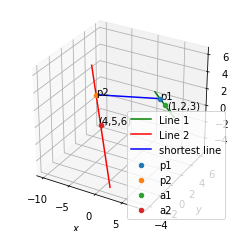
\includegraphics[width=\columnwidth]{solutions/sep/2/35/Figure/AS4.png}
    \caption{plot}
    \label{sep/2/35/fig:my_label}
\end{figure}

